\chapter{Background}
This chapter introduces the graph partitioning problem (GPP) and the objective functions used to evaluate partitions. It also reviews common practices in the field and gives examples of concrete application areas for graph partitioning (GP).

The first section defines the GPP and the central concepts that this thesis builds upon. The second section presents a short selection of graph partitioning algorithms, illustrating different approaches to tackling the problem. The third and final section discusses some of the most common applications of GP.

\section{Graph partitioning problem} \label{sec:gpp}
The GPP refers to a group of problems that deal with distributing the vertices of a graph into groups, clusters or communities. The goal is to group together vertices that are similar or that share many edges between them to minimize the number of edges among groups. The edges in some graphs are directed, meaning that they contain information about the communication flow among vertices. However, directed edges, or more generally directed graphs, are outside the scope of this thesis, and we consider only undirected ones.

Consider an undirected graph $G = (V, E)$ with $|V| = n$ vertices and $|E| = m$ edges. The goal is to partition $V$ into $k$ disjoint subsets $V_0, V_1, \ldots, V_{k-1}$ such that $V_i \cap V_j = \emptyset$ for $i \neq j$ and $\bigcup_iV_i=V$~\cite{karypis_multilevelk-way_1998}. The weight of the graph is $W = \sum_{v \in V}w(v)$, where $w(v)$ is the weight of vertex $v$ (vertices can also have multiple weights, but in this thesis we only consider graphs with a single vertex weight). Note that a graph with unit weights will have a weight equal to the number of vertices $W = n$. A balance constraint requires that all subsets have approximately equal weight. The weight of a partition is the sum of the weights of the vertices it contains: $w(V_i) = \sum_{v\in V_i} w(v)$. Using an imbalance parameter $\epsilon$, this constraint requires that each subset satisfies
\[
	w(V_i) \leq \left\lceil \frac{W}{k} \right\rceil \cdot (1 + \epsilon),\quad i= 0,1,\dots,k-1.
\]
The parameter $\epsilon$ represents the fractional excess weight a subset may have beyond the perfectly balanced weight $\lceil W/k \rceil$. When $\epsilon = 0$, the partition must be perfectly balanced~\cite{buluc_recent_2016}. The goal of GPP is to minimize a given objective function (see Section~\ref{subs:objective_functions}) while satisfying the balance constraint. GPP is NP-hard, meaning that for large graphs a solution can only be achieved through heuristics or approximation algorithms~\cite{garey_simplified_1976}. Unlike heuristics, which seek good solutions empirically without formal guarantees, approximation algorithms are required to come with a mathematically proven bound on how far their output can deviate from the optimum~\cite{Williamson_Shmoys_2011}. Despite their theoretical importance, approximation algorithms either underperform compared to state-of-the-art GP solvers or are too slow for large graphs~\cite{buluc_recent_2016}, making heuristics the most common choice in practice. 

Another common representation of scientific and engineering applications in GP is \textit{hypergraphs}. A hypergraph is a generalization of a graph where an edge, also called a hyperedge, can connect any number of vertices~\cite{buluc_graph_2013}. Similarly, GP divides the vertices into partitions while trying to maintain roughly equal size for each. However, given this more complex structure, utilizing hypergraphs requires more complex algorithms both in terms of implementation and running time. For the scope of this thesis, we will focus on standard GP; however, most of the techniques presented in this Section~\ref{graph_partitioning_algorithms} have been or can be applied to a solution based on hypergraphs as well.

\subsection{Objective functions}\label{subs:objective_functions}
An objective function is a mathematical formula used to define the goal of a problem, aiming to improve a specific value. The most common objective function in GPP is to minimize the total edge-cut~\cite{buluc_recent_2016}. An edge $\{u, v\} \in E$ is said to be \textit{cut} if its endpoints belong to different partitions, i.e., $u \in V_i$ and $v \in V_j$ with $i \neq j$. The total edge-cut is then the sum of all such cut edges across partitions. This also applies for graphs with edge weights, where the total edge-cut is then the sum of the edge weights of cut edges. 

Despite being a less precise measure of actual communication cost, edge-cut has been widely adopted as the standard objective function. Buluç et al.~\cite{buluc_recent_2016} attribute this to two factors: cut optimization appears to be easier in practice, and for graphs with high structural locality, the cut tends to perform similarly to other objective functions. 
%Additionally, alternative objectives complicate the use of multilevel approaches making them harder to implement.

Another common objective function is communication volume, which provides a more accurate measure of the data exchange between partitions of a communicating task. For a partition $V_i$, the outgoing communication volume is defined as $\text{comm}(V_i) = \sum_{v \in V_i} D(v)w(v)$, where $D(v)$ denotes the number of distinct partitions, other than the one containing $v$, in which $v$ has at least one edge to another vertex. The communication volume is then multiplied by the vertex weight, $w(v)$, as that represents the outgoing communication volume.

\subsection{Shortcomings of the objective functions}
Even though edge-cut is accepted as the standard, it comes with several shortcomings. Most notably, it does not distinguish between multiple edges connecting to the same neighboring partition. Consider Figure~\ref{fig:edge_vs_volume}, where each color represents a partition. Vertex $A$ has two edges, both leading to the blue partition. Calculating the edge-cut, $A$ contributes~2 to the total edge-cut. The communication volume, however, is only~1, since both edges connect to the same partition. In general, edge-cut can overestimate the actual communication burden, particularly for vertices with many neighbors in a single remote partition.

\begin{figure}[H]
	\centering
	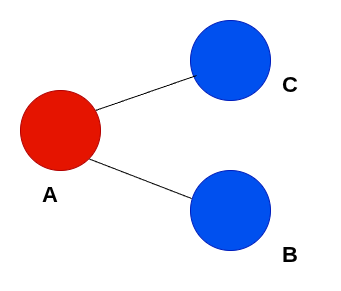
\includegraphics[width=.3\linewidth]{pictures/node_volume_1}
	\caption{Vertex $A$ has an outgoing communication volume of 1 but an edge-cut of 2. Each color represents a partition.}
	\label{fig:edge_vs_volume}
\end{figure}

The performance of a parallel application is generally limited by its slowest processor. This means that even if the computational work is balanced, the communication effort may not be~\cite{buluc_recent_2016}. In such cases, it is more meaningful to minimize the maximum communication load incurred on a single processor rather than the total load across all processors. Neither the standard edge-cut metric nor the total communication volume captures this type of objective.

Furthermore, on many architectures the time to send data, or messages, depends not on geographic distance but on the number of network switches the data must traverse. Although modern machines employ cut-through or wormhole routing to move individual messages quickly between distant processors, the communication network handles many messages simultaneously, and a message between distant processors occupies links that are unavailable to other traffic. Minimizing edge-cut does not account for this locality of communication, and a partition that places frequently communicating processors far apart in the network topology can lead to significant message contention~\cite{hendrickson_graph_2000, buluc_recent_2016}.

%Finally, the time to send a message on a parallel computer depends on both the latency (startup cost) and the message size. GP approaches typically aim to minimize the total communication volume but not the total number of messages sent. Depending on the machine architecture and problem size, message latencies can dominate message volume, making the number of distinct messages a relevant cost factor as well~\cite{hendrickson_graph_2000, buluc_recent_2016}. A few big messages might be more efficient than many small ones. 

%The choice of objective function becomes particulary consequential in the context of parallel computing which is discussed in detail in Section~\ref{}.
%Regardless of the objective function chosen, GP remains a fundamental tool across a wide range of domains. The following section discusses some of its most prominent application areas.
Regardless of the objective function chosen, GP remains a fundamental tool across a wide range of domains. The following sections discuss some of the most used GP algorithms and some of their application areas.

\section{Graph partitioning algorithms} \label{graph_partitioning_algorithms}
In this section we will present some of the most popular GP algorithms used today. The goal is to show some of the differences in the approaches and to highlight their typical use cases. This will help the reader to understand why the multilevel partitioning approach is deemed the best option for large scale graphs. These are, however, only \textit{some} of the existing GP algorithms; a more complete list can be found in~\cite{buluc_recent_2016, 10.1145/3571808}. 

\subsection{Recursive bisection} \label{recursive_bisection}
A popular partitioning method is recursive bisection (RB). Instead of partitioning a graph directly into $k$ subsets, RB first bisects the graph into two roughly equal parts using algorithms such as~\cite{barnard_spectral_bisection, fiduccia_fm, Kernighan_kl}, and then recursively bisects each part until $k$ partitions have been formed. When $k$ is not a power of two, modified schemes are used~\cite{simon_recursive_bisection, chan_spectralkway, KarypisGeorge1998AFaH, hendrickson_multilevel_1995}. Although simple and widely used, RB has been shown to produce suboptimal $k$-way partitions~\cite{simon_recursive_bisection}, since each bisection is made independently without knowledge of the cuts that will follow at deeper levels of the recursion. 

\subsection{Spectral bisection}
Spectral bisection was one of the first methods used to split a graph into two partitions and is still used today~\cite{buluc_recent_2016}. Its approach is to use the eigenvector, also known as the \textit{Fiedler vector}, of the second smallest eigenvalue of the Laplacian matrix to deduce global information of the connectivity of the graph~\cite{fiedler_eigenvector}. In order to form the two partitions, the median value $\overline{m}$ of the Fiedler vector is calculated, and every vertex with a value smaller or equal to $\overline{m}$ is assigned to one partition, and the rest to the other one.

The main computational cost of the spectral method lies in the calculation of the Fiedler vector. To optimize this, Barnard and Simon~\cite{barnard_spectral_bisection} have used a multilevel method to produce an approximation of the Fiedler vector. The spectral method has also been extended to produce a partition for more than only two partitions and to support edge and vertex weights~\cite{hendrickson_multilevel_1995}.

\subsection{Graph growing partitioning} \label{graph_growing}
Another bisection approach is called graph growing partitioning (GGP)~\cite{KarypisGeorge1998AFaH}. GGP is mainly based on breadth-first search (BFS). The core idea is to start from a random vertex and to use BFS to construct a partition. BFS is run until half the vertices are assigned to one partition, the remaining vertices are then assigned to the other one. The choice of starting vertex significantly affects the result, meaning that this algorithm tends to require multiple restarts to obtain a good solution. The GGP approach has also been extended to produce more than two partitions, called \textit{Bubble framework}~\cite{DIEKMANN20001555}. In this version $k$ starting vertices are chosen, evenly distributed in the graph. Starting from these vertices, \textit{k} BFS traversals are performed. Throughout, \textit{Bubble} uses local search algorithms to balance the partitions in the graph. At the end of an iteration, a new starting vertex is chosen for all partitions. The new starting vertex is the vertex with the minimum total distance to all other vertices in the same partition. The algorithm is repeated until no new changes occur in the choice of starting vertices, or no improvement for the partitions is found. The major drawback of this approach is its high computational cost.

\subsection{Streaming graph partitioning}
Streaming data models, where input is processed on the fly rather than all at once, have gained popularity due to their small memory requirements. In the field of GP, the input graph is also passed as a stream, requiring much less space than the graph size~\cite{buluc_recent_2016}. Streaming graph partitioning (SGP) is also very fast, even faster than multilevel algorithms (see Section~\ref{multilevel_gp}). However, these algorithms produce lower quality partitions compared to multilevel approaches. They are nonetheless useful in applications where speed is important, and an initial partition can be obtained from a stronger GP algorithm. For more details about SGP, we refer the reader to~\cite{stanton_streaming_gpp, tsourakakis_fennel, nishimura_streaming_gp}.

\subsection{Multilevel graph partitioning}\label{multilevel_gp}
Multilevel GP is considered to be the most successful heuristic for partitioning large graphs~\cite{buluc_recent_2016, KarypisGeorge1998AFaH, karypis_parallel_1999}. Because of this, multilevel GP was chosen as the base on which to build our new objective function NVOL. In short, the idea is that a graph is coarsened to a smaller graph. Once the graph is at its smallest, an initial partition is performed, and then it is iteratively uncoarsened to the original size. During the uncoarsening, heuristics are applied to improve the partitions. The intuition behind multilevel GP is that it is easy to run intensive partitioning algorithms on the small graph without affecting the total runtime. Additionally, starting from an already good solution, the refinement stage is not costly to perform and can quickly improve the partitions. Chapter~\ref{chap:multilevel-kway} will explain in detail the algorithm, providing the necessary background for understanding how NVOL is integrated into the framework.

\section{Applications of graph partitioning}\label{applications_of_gpp}
Graph partitioning arises in a broad variety of domains. This section highlights several of the most prominent application areas, though the list is by no means exhaustive.

\subsection{Parallel processing}
Perhaps the most widespread application of GP is distributing computational work across the processors of a parallel machine~\cite{langguth_load-balanced_2020}. GP is the standard approach in scientific computing applications such as sparse direct and iterative solvers. When the problem domain remains fixed throughout the computation, the partitioning can be performed once at the outset; this is known as static partitioning~\cite{buluc_recent_2016}. Other common applications in parallel processing include eigenvalue computations~\cite{boman_scalable_2013}, breadth-first search~\cite{buluc_graph_2013}, and algorithms for PageRank and connected components~\cite{salihoglu_gps_2013}. 

\subsection{Complex networks}
GP is also relatively popular in the field of complex networks~\cite{buluc_recent_2016}. Complex networks, in this context, refer to weighted graphs with nontrivial structure arising from real world or modelling processes~\cite{newman_networks_2010}. The objective functions applied in this field are usually domain specific, making it hard to develop optimization algorithms. 

Several application domains illustrate this breadth. In power grids, disturbances and cascading failures may lead to blackouts. GP can be used to isolate self-sufficient islands to prevent propagation of an outage~\cite{li_strategic_2005}. Cut based objective functions are sometimes extended to enhance the robustness of the system~\cite{li_power_2009}.

Geographically embedded networks have experienced a growth in requirements with the advances in
location-aware devices (such as GPS). It is now vital that algorithms be able to analyze networks like these extremely fast. In these networks the vertices commonly represent entities in the real world tied to geographic places. The cut-based approach therefore needs to be reinforced with spatial contiguity constraints~\cite{li_power_2009, buluc_recent_2016}.

Many biological systems can be modeled as graphs~\cite{buluc_recent_2016}, protein-protein interaction or gene co-expression graphs, for example. Partitioning serves multiple purposes ranging from data reduction to the detection of biological processes. More about this field can be found in~\cite{noauthor_wiley_2008}. 

In social networks, community detection is one of the most popular topics. In contrast to traditional GPP, the number of subgroups or partitions is not known a priori~\cite{buluc_recent_2016}. Apart from this, GP has contributed greatly to the development of community detection algorithms~\cite{fortunato_community_2010, newman_community_2013}.

\subsection{VLSI physical design}
VLSI circuit design has historically been one of the primary application areas for graph partitioning~\cite{buluc_recent_2016}. The objective is to decompose a circuit into smaller subcircuits, ranging from gate arrays to complete integrated circuits, while minimizing the total interconnection cost, typically measured as the weight of connections crossing partition boundaries. In this formulation, nodes represent cells (i.e., basic logic or functional units such as gates) and edges represent wires. Scalability is essential, as circuits can contain millions of modules and partitioning constitutes a bottleneck in the overall design flow. Beyond the basic cut objective function, practical VLSI partitioning must also respect domain specific constraints such as I/O placement, groups of cells that are required to remain in the same block, and upper bounds on the cut size between block pairs. Further details can be found in~\cite{kahng_vlsi_2011, cong_multilevel_2003}.

\subsection{Neural networks}
Graph neural networks (GNNs) extend deep learning to graph structured data, enabling the processing of irregular domains that traditional neural network architectures cannot readily handle. However, as graph sizes grow, training GNNs becomes increasingly expensive due to rising communication overhead, particularly in distributed or multi-device settings. Graph partitioning offers a natural approach to this scalability challenge by distributing subgraphs across devices while minimizing inter-device communication.

A recent example is CaPGNN~\cite{song_capgnn_2026}, a parallel full batch GNN training framework designed for multi-GPU servers. CaPGNN combines resource aware graph partitioning with an adaptive caching mechanism that exploits both CPU and GPU memory to reduce redundant data transfers. By taking into account the heterogeneous computational and communication capacities of individual GPUs, the framework achieves substantial reductions in training time with minimal impact on model accuracy. While this is only one instance of a broader trend, it illustrates how classical graph partitioning techniques are finding renewed relevance in the context of modern machine learning workloads.

Another recent example is ParDNN~\cite{qararyah_computational-graph_2021}, an automatic, generic, and non-intrusive partitioning strategy for deep neural networks represented as graphs. Like CaPGNN, this strategy has the goal of minimizing the training time of the model without affecting accuracy. Through their experiments, Qararyah et al. how significant improvements over related work in efficiency, batch size scaling, and training throughput.

